% This file should be replaced with your file with an thesis content.
%=========================================================================
% Authors: Michal Bidlo, Bohuslav Křena, Jaroslav Dytrych, Petr Veigend and Adam Herout 2019

\chapter{Introduction}
importance of GUI testing, goals, regressions, errors 

The goal of this work is to design and implement a tool for generating tests for GNOME desktop applications using AT-SPI metadata created as a by-product of an architecture supporting assistive technologies.

The architecture expose application as a tree of accessibility objects with their current state. Every object is defined by several properties and set of actions that can be invoked to change the current state. Since accessibility support has been implemented to very fundamental layers of GTK/GNOME framework (widget level), it provides a suitable way for development of automated test suites.\cite{pyatspi2} 

Modern GUI applications are being developed more rapidly with lack of proper regression testing. 

manual testing vs automation clanok

Additionally this effort should also help to reveal defects and missing parts in accessibility itself and improve the experience for users with disabilities.

\chapter{Accessibility}
Accessibility in general is a technology that helps people with disabilities to participate in essential life activities. Considering the accessibility as a part of GNOME desktop, it includes libraries and development tools allowing users with disabilities to use other options of interaction with GNOME desktop environment. Those options includes voice interfaces, screen readers and other alternative input devices.\cite{gnomeADG}
\section{The Accessibility Toolkit (ATK)}
Assistive technologies are receiving information from the Accessibility toolkit (ATK) which provides built-in API for all GNOME widgets. ATK provides a set of interfaces which are required to be implemented by GUI components. Therefore, assistive technologies are able to automatically read most of the labels on screen without any extra efforts made by developers. The interfaces are toolkit-independent, meaning that their implementation could be written for many widgets, including widgets from frameworks such as GTK\footnote{https://www.gtk.org/} and Qt\footnote{https://www.qt.io/}.
\section{GNOME Accessibility Implementation Library (GAIL)}
Majority of GNOME applications are written in GTK framework. The framework provides dynamically loadable module named GAIL implementing ATK interfaces for all GTK widgets. Once the module is loaded at runtime, the application is fully capable to cooperate with ATK without any further modifications.
GNOME desktop does not load accessibility support libraries by default, it has to be enabled by setting a special gsettings key which can be achieved either by dconf\footnote{https://wiki.gnome.org/Projects/dconf} editor or by execution of the \texttt{gsetting} command in terminal:
\begin{verbatim}
    gsettings get org.gnome.desktop.interface toolkit-accessibility true
\end{verbatim}
Additional configuration may be required for applications written in other frameworks such as QT or Java. Furthermore, implementations of other assitive technologies might be too application specific or use various techniques like OS event snooping etc. Compared to GNOME Desktop, all information required by assistive technologies (AT) are passed from GNOME Accessibility Framework to a toolkit-independent Service Provider Interface (SPI). The SPI is a key component providing stable and consistent API for screen readers, magnifiers, etc. Accessibility support is relying on per-toolkit implementation (GTK, QT, Java) and its APIs exported through relevant bridges to unified AT-SPI interface, as described on Diagram \ref{ATSPI_architecture}.

\begin{figure}[hbt]
	\centering
	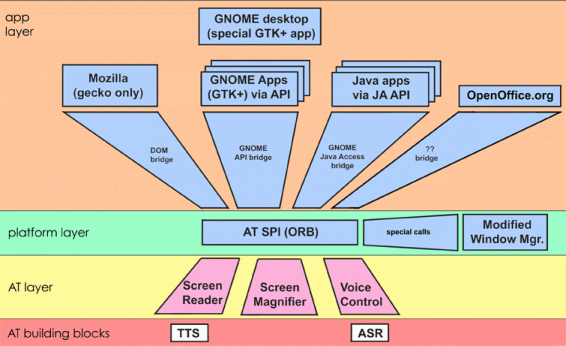
\includegraphics[width=1\textwidth]{obrazky-figures/GNOME_desktop_Accessibility.png}
	\caption{GNOME Accessibility Architecture overview}
	\label{ATSPI_architecture}
\end{figure}

The widget is accessible, if a developer use any GTK/GNOME widget and follows the general accessibility guidelines\footnote{https://developer.gnome.org/accessibility-devel-guide/stable/gad-coding-guidelines.html.en} with properly implemented ATK interfaces. Considering that the stock GTK/GNOME toolkit widgets have implementations of these interfaces provided, new widgets will inherit the functionality and gain suitable accessibility support as well. The default implementation of ATK interfaces might be altered by applications, as developers may improve their descriptions of widgets and improve the user experience in special cases when widget is used for some less expected purposes or the default description is too general. The ATK provides set of functions to achieve this along with the ability to make any custom component accessible\footnote{https://developer.gnome.org/accessibility-devel-guide/stable/gad-custom.html.en}.\cite{accessibleWidgets}

\newpage
\section{Library pyatspi}
Package pytaspi is a Python wrapper around AT-SPI C implementation which loads the Accessibility typelib and imports the classes implementing AT-SPI interfaces.\cite{pyatspi}

AT-SPI exposes applications as a tree of widgets starting with a root element where every sub-element represent one running application on the GNOME desktop. Each application has zero or more children, each child is distinguishable by its position in the tree and several properties including:
\begin{itemize}
    \item name - string value, for most widgets contains text identical with a text label visible on widget
    \item roleName - string value, specifies the widget type
    \item childCount - integer value, a number of sub-elements 
    \item actions - list of strings, contains available actions which can be performed by the ATK
    \item visible - boolean value, indicated that object is visible to the user
    \item showing - boolean value, object is rendered
    \item text - string value, mostly used in input fields or widgets containing plenty of text
    \item description - string value, contains special widget description for users
    \item position - integer tuple, x, y coordinates on the screen (might be related to other component)
\end{itemize}

Additionally, elements can be linked together in other useful ways (except parent-child relationship) where labels are linked with widgets like text fields, check boxes, combo boxes etc. These labels are making widgets easier to find or interact with. Other advantageous properties like showing or visible can be used to decide whether elements are hidden from the active screen area, thus they are not available for interaction. Role names of elements are also important as some elements are offering some widgets specific methods like selecting values in radio buttons, selecting options in combo boxes or a simple click method on push buttons. Access to this functionality is focused in a singleton object named registry that provides services for subscribing to specific events and as mentioned before, generating mouse and keyboard events on demand.

pyatspi is an open source project available for most of Linux distributions via distro specific packaging services (package named python3-atspi) or can be built from its sources\footnote{https://gitlab.gnome.org/GNOME/pyatspi2}.

\section{Expoloring and Debugging the Accesibility}
Currently, there are several tools available for exploration and debugging accessibility features not only on GNOME desktop. 
\subsection{dogtail}
Dogtail is an open source GUI test framework written in Python implemented as a library around pyatspi. Several modules implements another(higher) level of API to simplify work and interaction with accessible objects during test development. The tool offers less complex functionality, containing tree view of objects with their basic attributes\cite{dogtail_doc}. Dogtail package also includes a GUI tool Sniff, similar to the Accerciser application but described in the next section
The most important dogtail framework modules are:

\begin{itemize}
    \item tree - the module contains the most important class Node, instances of node class represent elements of the desktop user interface, all elements are gathered to tree structure representing all applications starting with the root element(desktop), the node class is implemented as a mixin for Accessible and various Accessible interfaces and is an important unit for it's subclasses, namely Application, Root and Window, the class also implements methods allowing to search for nodes in the tree based on certain criteria, including element properties name, rolename, showing and visible. Furthermore, it implements action methods that can be performed on the nodes without importing other modules, there is also a blink method, once it is called element is highlighted on the screen. This functionality is also part of the Sniff tool where element is highlighted after it is selected in the tree.    
    \item dump - dumping tree of nodes as a plain text, useful for python/ipython console debugging
    \item rawinput - contains implementation required for generating events from both keyboard and mouse, including more complex events like keyboard shortcut events and mouse gestures to emulate drag and drop operations  
\end{itemize}

 \begin{figure}[hbt]
	\centering
	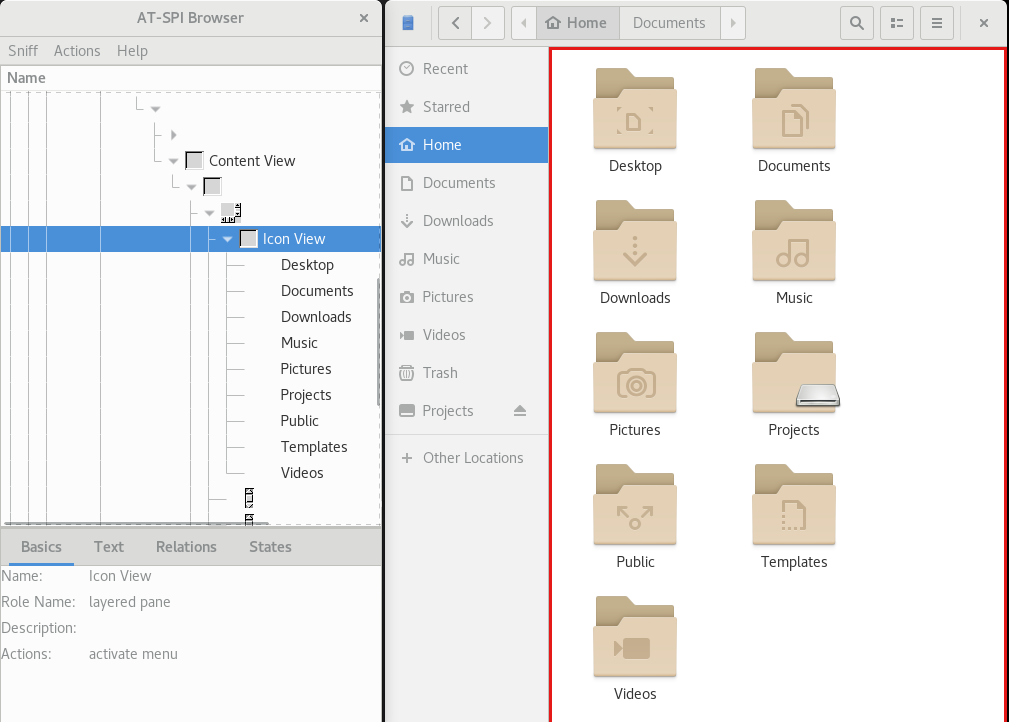
\includegraphics[width=1\textwidth]{obrazky-figures/sniff.png}
	\caption{Sniff utility highlighting icon area in Nautilus File Manager, Screenshot taken from Red Hat Enterprise Linux 8.2}
	\label{sniff}
\end{figure}

 Testing Dogtail has proven availability for many Linux distributions through their package repositories, specifically Fedora 32, Red Hat Enterprise Linux 8.2 and Manjaro 18 with GNOME 3.34 (Archlinux). It is also available as a Pypi Python package and according to information in it's official Gitlab repository should work not only for GTK+ application but also for application written in QT and KDE4. 
 
 Dogtail testing reveals also some minor problems which might occur during the test development, to be more specific the were cases when the coordinates of a node were not reported correctly. Some items are not labelled with names like panels and lists, those are mostly items that are not as important for user interaction as their are not containing any text but they are still accessible as they are parents for other elements of the UI. Unfortunately the testing discovered also some of the important buttons to be more specific menu buttons that are nameless. Once an action needs to be dispatched on such element it is required to use its parent or sibling element for identification and for actions performed by mouse make an adjustment of the coordinates, so it can be performed on the right node. So to conclude this chaper, dogtail is powerful tool for development of automated testing but it also has it's bug and limitations. Those limitations mustn't come from the dogtail itself but it might be caused either by accessibility bugs or just not respecting the accessibility guidelines during the development of the custom widgets. 

\subsection{Accerciser}
Accerciser is an interactive accessibility explorer developed in Python. It provides well-arranged graphical frontend for AT-SPI library, hence it can inspect, examine and interact with widgets and also allows developers to verify that their applications are providing correct information to assistive technologies and automated testing frameworks. The default interface has three sections: A tree view with the entire desktop accessible hierarchy and two optional plugin areas. Accerciser has an extensible, plugin-based architecture, most of the features available by default are part of the following plugins\cite{accerciser}: 

\begin{itemize}
    \item Interface Viewer - explorer of the AT-SPI interfaces provided by each accessible widget of a target application, after an item is selected, interfaces shown for the selected item will become sensitive, so all methods can be executed, including methods for object interaction like click and other methods for retrieving more object information. Accerciser allows to explore the following interfaces:
    \begin{itemize}
        \item Accessible - show child count (number of child widgets), description, states, relations and other attributes
        \item Application - if implemented (not mandatory), it shows application ID, toolkit and version
        \item Component - shows item's absolute position with respect to the desktop coordinate system, relative position with respect to the  window coordinate system, size, layer type, MDI-Z-order indicating the stacking order of the component and alpha
        \item Document - shows document attributes and locale information
        \item Hypertext - shows a list with all item's hypertext links,  including name, URI, start index and end index
        \item Image - shows item's description, size, position and locale
        \item Selection - shows all selectable child items of the selected item,
        \item Streamable Content - shows selected item's content type and their corresponding URIs
        \item Table - shows item's caption, rows, columns, number of selected rows, number of selected columns and for selected cell, it shows  it's row's and column's header extents  
        \item Text - shows selected item's text content, that can be editable with attributes offset, justification  and possibility to show CSS formatting as well
        \item Value shows item's value, minimum value, maximum value, minimal increment for a value 
    \end{itemize}
    \item AT-SPI Validator - applies tests to verify the accessibility of a target application, the validator will generate the report of the selected item and all its descendant widgets in the tree hierarchy
    \item Event Monitor - displays AT-SPI emitted events, it also provides the filter for several different AT-SPI event classes with the ability to monitor only events sourced from selected application or selected accessible(widget), each event record contains the source and the application.
    \item Quict Select - provides global hotkeys for quickly selecting accessible widgets in Accerciser's Application Tree View, selected widget is highlighted in the target application
    \item API Browser - shows interfaces, methods and attributes available on each accessible widgets of a target application, by default it shows only public methods and properties, private methods and properties are hidden until checkbox \texttt{Hide Private Attributes} is unchecked
    \item IPython Console - full, interactive Python shell with access to selected accessible widgets of a target application, use full debugging tool especially in combination with the Interface Viewer
\end{itemize}

\begin{figure}[hbt]
	\centering
	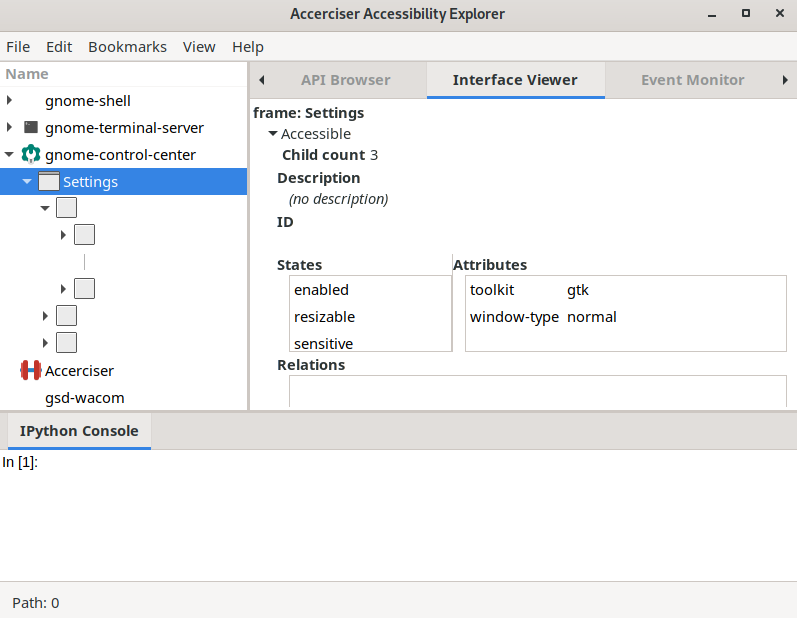
\includegraphics[width=1\textwidth]{obrazky-figures/accerciser.png}
	\caption{Accerciser default configuration, Screenshot taken on Manjaro Linux with GNOME 3.34}
	\label{Accerciser}
\end{figure}

\chapter{GUI TESTING}
https://ldtp.freedesktop.org/wiki/
https://en.wikipedia.org/wiki/Linux_Desktop_Testing_Project
https://wiki.ubuntu.com/Xpresser/
AppStream data
\chapter{python}
\chapter{behave}
\chapter{Covering Limitations of Accessibility and Verification}
As discussed in aforementioned chapters information provided by accessibility is not flawless, therefore next couple chapters are dedicated to exploration of technologies that might be used to support the accessibility in such cases.

\section{OpenCV - image matching}
OpenCV or Open Source Computer Vision Library is a software library that provides optimized algorithms for computer vision and machine learning. According to official OpenCV webpage\cite{opencv}, the library contains more then 2500 algorithms and it is being developed 
by a vast community of contributors around the world. The library is used extensively bu government institutions, research groups and companies including Microsoft, Google, IBM and many more. One of the biggest advantages is its native C++ implementation with bindings making the library available in Python, Java and Matlab and supports Linux, Android, Mac OSX and Windows. Regardless of Linux distribution, similarly to dogtail, OpenCV can be installed easily via python3 package manager(pip). 

From the rich availability of algorithms provided, an image recognition algorithm can be used to either locate of verify the presence of an element on the screen. This approach would require to have and image of the element prepared in advance, then it can be used to find the image location on the screenshot of the screen taken during a test run. Compared to verification of the node only via accessibility, this approach would also verify that the element is properly rendering on screen and the shown result is really an element that has to be shown to the user with verification of text formatting and colors. On contrary, there this process requires additional manual work of taking images, labelling them and associating them with certain test scenarios. Additionally, more complications might appear as some of the elements may be displayed on the screen multiple times which would make a count of items on the screen at the same time another compulsory parameter that is required to maintain. The most common example of such case are buttons labelled either OK or Cancel as they are used in many applications.

Another possible approach is to use the shape recognition algorithm which can locate shapes like circles, rectangles any many other common shapes. From the development perspective this would be easier to maintain as there is no requirement for images prepared in advance(compared to image recognition algorithm) but can help with the widget location in cases where accessibility is reporting wrong coordinates. On the other hand, locating the right widget in cases when several similarly shaped ones are located on the screen at the same time will yield very inconsistent results.


\section{OCR}
Optical Character Recognition or OCR is a method of extracting text from images. One of available open source tools is a tool called Tesseract.

Initially, Tesseract development started in 1985 at Hewlet Packard Laboratories but the major breakthrough was achieved in 2006 when the project was open sourced in cooperation with University of Nevada in Las Vegas. Since then the project has been developed under the sponsorship of Google\cite{tesseract_history}.

Usability of Tesseract was increased in version 3.x, supporting wide range of image formats and gaining ability to be used in larger number of scription languages. While Tesseract 3.x is based on traditional computer vision, in the past few years methods based on Deep Learning have surpassed traditional machine learning techniques by vast margin, especially in terms of accuracy in several areas of Computer Vision. Remarkable results were achieved in handwriting recognition. Tesseract has implemented a Long Short Term Memory(LTSM) based recognition engine is a kind of Recurrent Neural Network (RNN). This kind of RNN is used to recognize an image containing a text of random length meanwhile a Convolutional Neural Network is used for recognition of single character. Version 4 provides both legacy OCR engine and new LSTM engine which is enbaled by default.\cite{tesseract}

Tesseract can be used as a command line tool, integration in development is possible via Tesseract's API available in python or C++. Setup on Linux or other platforms may differ but the process is accurately described in Tesseract's wiki\footnote{https://github.com/tesseract-ocr/tesseract/wiki}, the last resort solution is to built it from its sources.
The setup process includes installation of tesseract-ocr package itself, pytesseract python bindings installable via python's package manager pip and Tesseract's language pack with trained data for English language(version 4.x supports 130 languages\footnote{https://github.com/tesseract-ocr/tesseract/wiki/Data-Files#data-files-for-version-400-november-29-2016}). 

Tesseract's OCR engine works best when used on images with clean black text with white background in a common font. Text should be approximately horizontal with the height of at least 20 pixels. Surrounding border around the text can be detected as some random text. With possibilities of image processing provided by OpenCV, the image quality in some cases need to be improved before applying text detection methods. Most common image preprocessing methods include inverting images, rescaling, binarisation, noise removal, rotation, border removal and page segmentation\footnote{https://github.com/tesseract-ocr/tesseract/wiki/ImproveQuality}.

Tesseract's API for python is bundled in a module named \texttt{pytesseract}. The module provides several methods, the most important ones for the purposes of this \verb|image_to_string| and \verb|image_to_data|. Both methods have one compulsory parameter which is an image intended for text extraction. Image has to be in certain format, one of the option is to load image through OpenCV's \texttt{imread} method. Additional parameters may be applied including language, timeout and engine configuration\footnote{https://pypi.org/project/pytesseract/}. The first method returns all recognized strings including all whitespaces and other special characters. The second method provides additional metadata about all recognized strings in a form of dictionary like object. The returned dictionary contains the following lists of properties:

\begin{itemize}
    \item text - string value, may contain string, special character, one word or line of text
    \item left - integer value, specifies number of pixels from the left side of the image 
    \item top - integer value, specifies number of pixels from the top of the image
    \item width - integer value, specifies width of the recognized string 
    \item height - integer value, specifies height of the recognized string
    \item the rest are less important values for this work: \verb|level, page_num, block_num par_num| \verb|line_num, word_num, conf|
\end{itemize}

Therefore, occurrences of certain string in an image can be filtered and highlighted in every image as demonstrated on Figure \ref{ocr_nautilus} for string \verb|Documents|.

\begin{figure}[hbt]
	\centering
	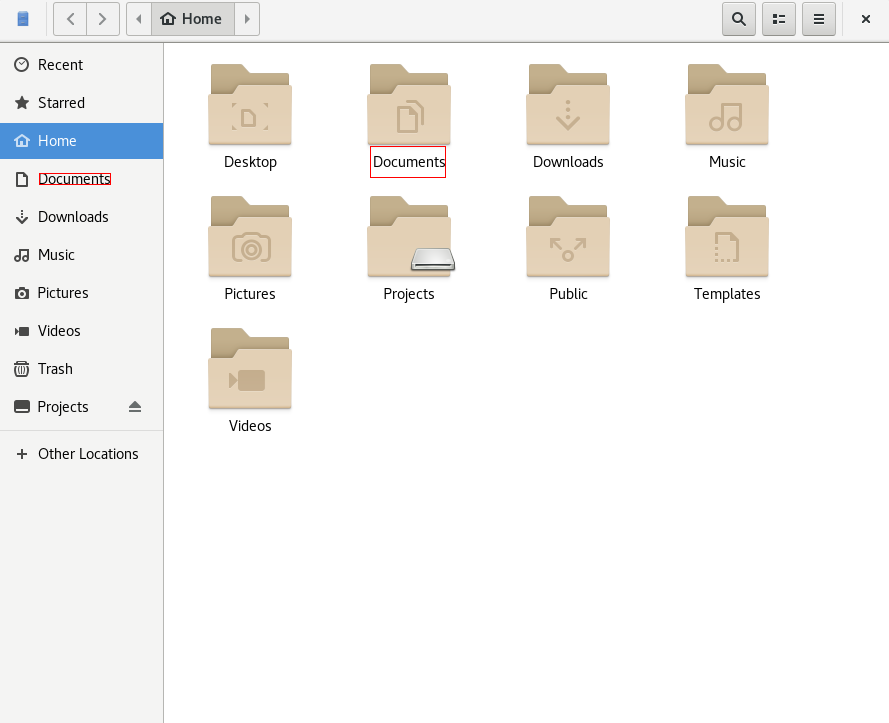
\includegraphics[width=1\textwidth]{obrazky-figures/ocr+nautilus.png}
	\caption{Demonstration of the OCR engine detection for the string Documents in Nautilus File Manager Window, Red Hat Enterprise Linux 8.2}
	\label{ocr_nautilus}
\end{figure}

Similarly to OpenCV, Tesseract's OCR engine was tested as an alternative tool for location of verification of widgets which contain text. This method also verifies that the content was properly rendered and is readable for user. Preprocessing might be required for some cases, considering different text background in some applications due to different color theme or just highlighted text can cause problems for the OCR engine. Those cases can be solved by before mentioned image preprocessing methods provided by OpenCV. 

\section{Conclusion}
This chapter evaluated technologies that may be able to cover limitations and bugs in accessibility. Both OpenCV and Tesseract may help with identification, location and verification of non-accessible elements in applications and they depend on screenshots of applications that need to be taken in the right time. OpenCV's image matching algorithm can reliably locate prearranged images of icons, labels or whole application on the screen. Considering the stable application environment with black text on white background in most of applications, Tesseract is able to detect and reliably locate most of the text content on the screen. Furthermore, both technologies are working with actual appplication content rendered to users which can bring additional level of verification.